\subsection{General Language Characteristics}\label{sec:langcharacteristics}
As illustrated in \figref{fig:languagefeatures}, we identified the following general characteristics in which the languages differ, represented by the features \fnotation, \fsemantics, \flangparadigm, and \fextensibility. The actual concepts offered by the languages will be discussed in \secref{sec:langconcepts}.

%The language sub-feature, figure  \ref{fig:languagefeatures}, identifies five features from which four are mandatory: language concepts, notation, semantics and language paradigm. While the extension feature (21/29) is an optional feature. Some languages support extension of the language functionalities by any user especially those which are open-source  while other do not.

%The language constructs for motor, and sensor  data configurations are abstracted closer to those who are familiar to the use of the sensor than just robot engineers. For example \emph{set motor speed, obstacle detector event block (grey: ignore detector, white: object close and black: object far)}. \claudio{The previous sentences are part of the methodology} The fact that these languages support graphical notations breaks the barrier created by text notation among novice programmers, as asserted by Fernandez-Permomo et al.\cite{Fernandez-Perdomo2010}, hence increasing usability, learnability and satisfaction among end-users. \claudio{Not clear what is the point of this sentence? Here we should discuss the FM we have created}
%\tb{we need examples of domain-specific terminology in the languages, can you provide some? also, examples why you think the languages are end-user facing; why is that the case?}
%For instance, they support end users through \dots. Most (X\,\%) are also graphical.
%domain, which generalized features that support novice programmers and robotics domain, which take care of technical features for professionals in robotics or software engineering.
All the languages identified in the environments including the textual ones have been customized to support the robotics domain, for example, by introducing domain specific actions. Some of the actions in \lego are stop motors, play tone in \trik, set robot's state, set top color in \aseba,  drive straight, and turn right. %in \lego are some domain specific actions.% \tb{how? give examples of domain-specific keywords and domain-specific graphical elements}.

\begin{figure}[t]
     \centering
    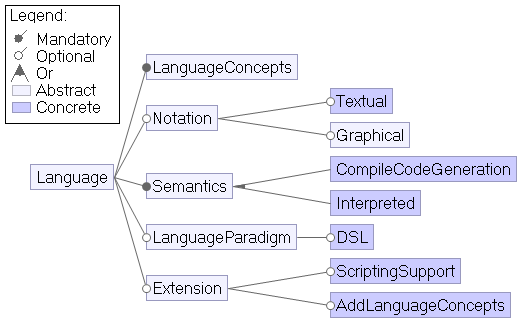
\includegraphics[width=.75\columnwidth]{Languagefeatures.png}
      \caption{Language Characteristics}
      \label{fig:languagefeatures}
   \end{figure}

\parhead{\fnotation.} All the environments offer languages with a domain-specific visual notation (concrete syntax) for their end-users. The textual and visual notations offered by the respective environments are summarized in \tabref{notation}.

We classify the notations into:

\begin{itemize}
	\item \f{Tree-Based} syntax, as realized using the Blockly or Scratch libraries (cf. \secref{sec:background}). An example of the former is shown in \figref{metabot}, and of the latter in \figref{scratch-marty}. But, this kind of syntax is also realized with own implementations in some environments, such as \robotc, as shown in \figref{fig:robotcgraphical}.
	\item \f{Graph-Based} syntax, such as in \choregraphe (cf. \figref{fig:choregraphe}, %Flowol in
	\robotmesh, and %flowchat in
	\picaxe, which use connectors between nodes (blocks) to form graph-like structures. 
	%\item forms and tables as shown in Figure \ref{fig:robotcgraphical}
	\item \f{Custom} syntax. For instance, \flyaq offers a map-based mission language to specify (drone monitoring) missions by clicking on locations where tasks shall be executed. \aseba essentially has vertical lists of even-action pairs, as shown in \figref{fig:aseba-vpl}. Finally, we found customized block diagrams such as in \lego, as shown in \figref{fig:legoloopcount}, which is essentially a graph, but we classified separately due to the different kind of connectors (blocks are adjacent when connected, not using line edges).
\end{itemize}


Almost every syntax
%(\tivipe is an exception, for instance)
is customized with robotics-domain-specific figures, such as icons. For instance, a block \emph{Motor forward} in \trik has a gear icon with a forward arrow depicting a forward-running motor. The user only specifies the motor power and the port in which the motor connects. 13 of our environments additionally offer a textual syntax, often by just allowing the use of a general-purpose language in parallel to the primary visual DSL. Some environments use a mix of textual and visual notations, like \easyc, as shown in \figref{fig:easyc-sidebyside}.

\begin{figure}[t]
\vspace{-.4cm}
     \centering
    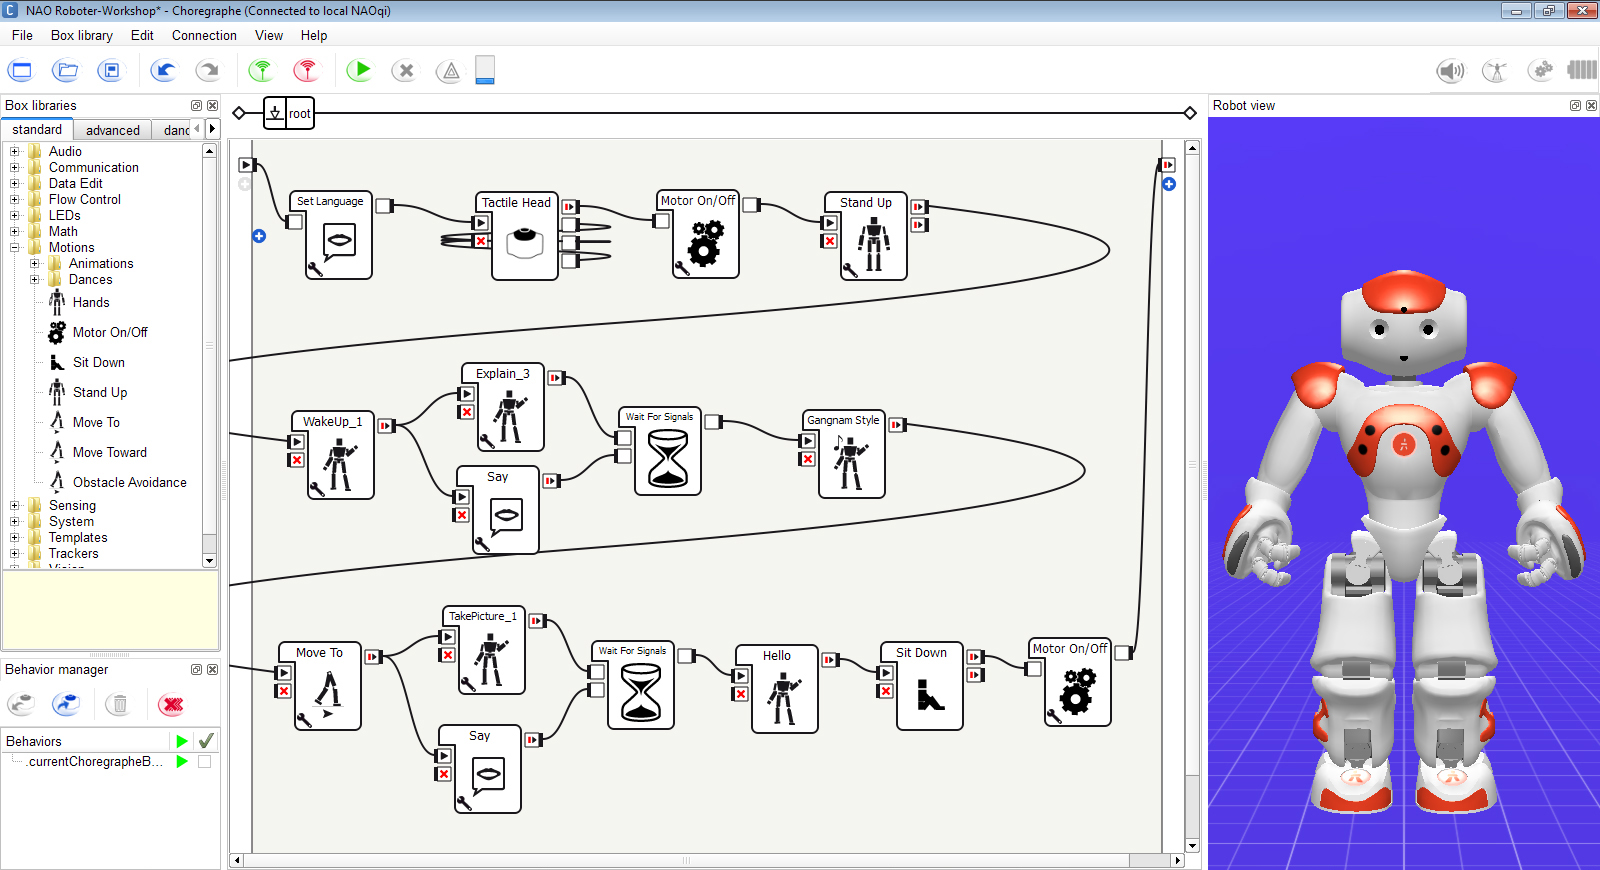
\includegraphics[width=\columnwidth]{fig/examples/choregraphe.jpg}
      \caption{The environment \choregraphe for the robot NAO}
      \label{fig:choregraphe}
			
   \end{figure}


%\tb{do you know for how many the textual syntax belongs to the same language (the main, visual language) and for how many it is a separate language (which could also be a gpl)?}.


%\tb{but thought we have graph-based and block-based as our features?}
%\begin{itemize}
%	\item Blockly-based as shown in figure \ref{metabot}%\tb{characterize what you've seen; how does it look like}
%	\item Scratch-based as shown in figure
%	\ref{scratch-marty}%\tb{characterize what you've seen; how does it look like}
%	\item forms and tables as shown in figure \ref{fig:robotcgraphical}%\tb{characterize what you've seen; how does it look like}
%	\item textual where End-user codes a mission using text characters.%\tb{characterize what you've seen; what kinds of textual notations do we have? how do they look like?}
%\end{itemize}

%, or make use of tables and forms, as \robotc as shown in  %\figref{fig:robotctextual} and 

\begin{figure}[b]
	\centering
	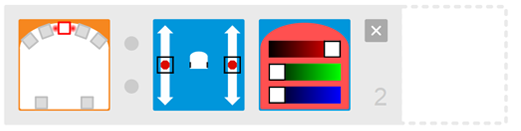
\includegraphics[width=\columnwidth]{fig/aseba-vpl-event-action-pairs.png}
	\caption{\aseba's visual notation for its language VPL, which is an event-based language consisting of event-action pairs. One such pair is shown here.}
	\label{fig:aseba-vpl}
\end{figure}


%Textual: \edison, \choregraphe, 
%%\tb{choregraphe is definitely visual!},\swaib{the point is it also supports textual notations} 
%visual: \minibloq, \trik, \choregraphe, and mix of both text and visual \easyc \figref{fig:easyc-sidebyside} or by use of tables and forms as provided by \robotc in  %\figref{fig:robotctextual} and 
%\figref{fig:robotcgraphical}. % \tb{add screenshot}.
%The notations offered by the respective environments have been summarized in the table \ref{notation}.

%- symbol shapes in graphical notations
%- Blockly library: It has been implemented in various environments as shown in table \ref{notation}% Roberta\,\cite{OpenRoberta,PICAXE,RobotMeshStudio} \tb{make complete, where else?}

\begin{figure}[t]
	\centering
	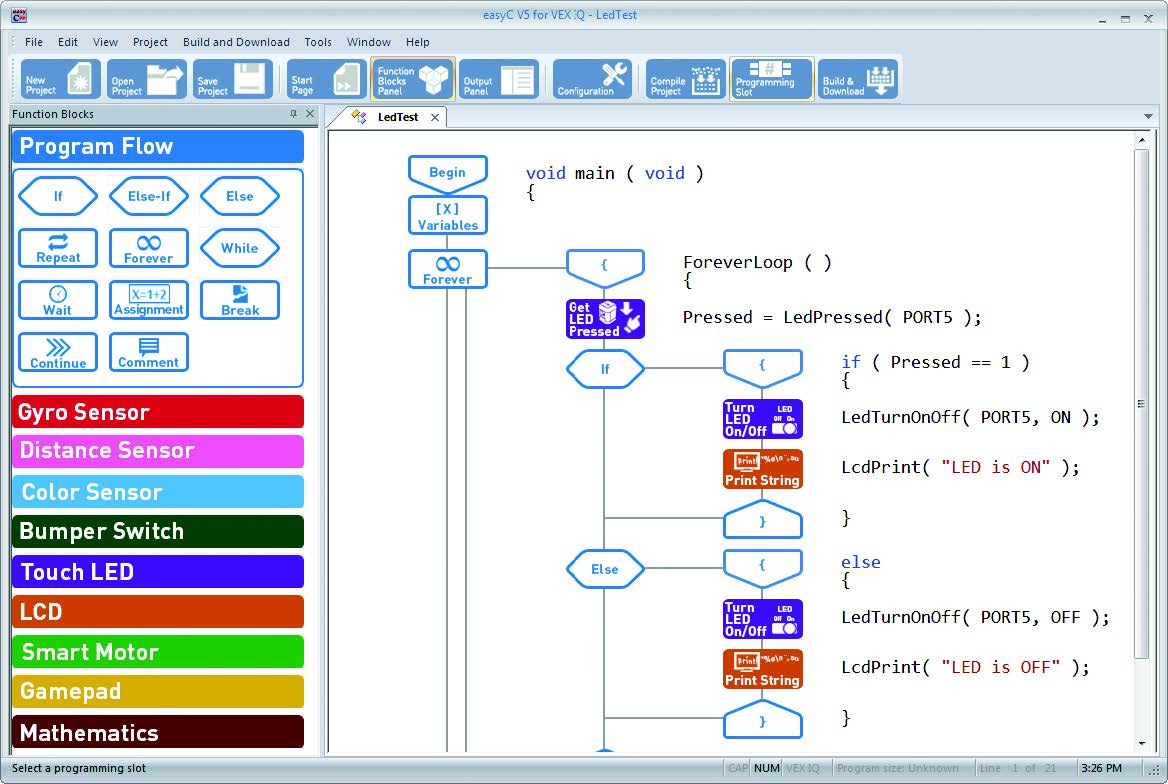
\includegraphics[max size={0.5\textwidth}{\textheight}]{projectionalEasyC.jpg}
	\caption{Graphical and textual syntax side-by-side in \easyc's projectional editor%\tb{TODO: create better screenshot}
	}\label{fig:easyc-sidebyside}
\end{figure}

% \begin{figure}[t]
% 	\centering
% 		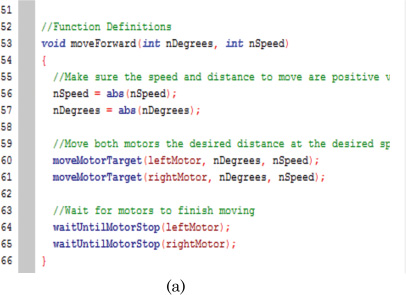
\includegraphics[max size={0.5\textwidth}{\textheight}]{robotCtext.png}
% 	\caption{RobotC, (a) textual \cite{Schunn2017} }
% 	\label{fig:robotctextual}
% \end{figure}

\begin{figure}[t]
	\centering
		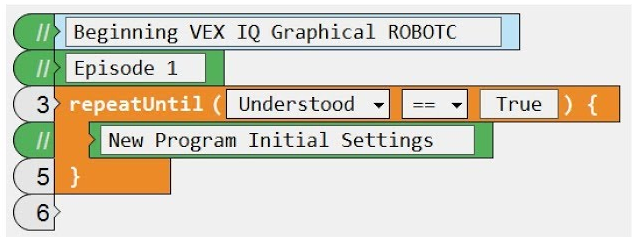
\includegraphics[width=.8\columnwidth]{robotc2.png}	\caption{\robotc's visual notation (from \cite{Admin})}
	\label{fig:robotcgraphical}
	\vspace{-.4cm}
\end{figure}
%\claudio{Missing verb. Which details?} %Secondary notation services provide extra information on the marks and cues used for specification of missions, like; comments, and size of blocks~\cite{Blackwell2001}.

\begin{table*}
\caption{Kinds of notation supported by the environments (the graphical notations belongs to the primary DSLs of the environments; the textual ones to additional languages supported, which can be a GPL)}
\label{notation}
\begin{tabular}{ m{3cm}m{13.6cm}}
\toprule
\textsf{notation} &\textsf{environment}\\
\midrule
\textbf{graphical} &\\
Blockly-based & \picaxe, \ardublockly, \openroberta, \arcbotics, \aseba, \robotmesh, \blocklyprop, \ozoblockly, \turtlebot, \makecode, \robotc \\
Scratch-based & \edison, \aseba, \sphero, \vex (modkit), \marty, \makeblock, \codelab, \tello, \scratchev, \enchanting, \\
Control-flow graph & \picaxe (flow chart), \missionlab, \tivipe, \choregraphe (flow diagram), \robotmesh (flowol), \trik \\
Custom & \edison(EdBlock), \flyaq (map), \aseba(custom blocks with icons, see \figref{fig:aseba-vpl}), \codelab (icons), \lego(icons), \minibloq(icons), \easyc\\
\midrule
\textbf{textual}&\\
C/C++ & \arcbotics, \vex, \robotmesh, \trik, \easyc\\
Python & \edison, \robotmesh, \marty, \makeblock, \trik, \codelab\\
%Java & \patrizio{empty here? Remove?}\\
JavaScript & \picaxe, \sphero, \marty, \trik \\
Custom & \picaxe (custom language in the style of Basic), \ardublockly (Arduino C), \aseba (custom event-based language) \\
\bottomrule
\end{tabular}
\end{table*}



\parhead{\fsemantics.} The semantics of our languages are determined by either interpretation or compilation (target code generation). The mission specified is either semantically translated (compiled) as shown in \tabref{tab:codegentable} or interpreted to preserve what is specified and what the robot actually executes. Apart from \lego and \codelab, whose missions are interpreted, all the other 27 environments generate code. \metabot directly generates assembler code, while the rest compiles generated code. \trik, which supports multiple robots (Lego EV3, Lego NXT, Pioneer Kit, and the TRIK robot), while it does not cross-compile, since missions are robot specific, it generates code in various target languages, including C, JavaScript, Pascal, Python, and F\#.

%In the case of Lego EV3, missions are interpreted, with support for both USB and Bluetooth connections. % -> don't understand

%In the case of Lego NXT, besides interpretation, \trik generates C  code

%language\tb{what is that? can you give me a reference to that language?} and NXT OSEK C language\tb{what is that? can you give me a reference?} \swaib{I saw Russian C and OSEK C languages as possible languages for generated code for the when running \trik. My best reference is when you install \trik. But I have not seen published documentation about them}, while in the case of TRIK robot, the environment generates Java Script, PascalABC, Python, and F\#.%\tb{why does it generate programs in so many different languages?} \swaib{Russian C, OSEK C are target languages seen in the list, however there is no much documentation about them in the tool documents. I have not figured out why TRI robot missions can be generated into several languages}. \codelab provides support for mission interpretation using Python SDK\tb{unclear, what does that mean?} \swaib{the interpreter was built using python software development kit (SDK)}.

% \begin{table*}
% \caption{Code generation matrix indicating languages of generated code from the graphical notations\tb{remove the classification according to the notation, just have a two-column table: first column: target language, second column: environment generating it; use the other tables' style}}
% \label{Codegeneration}
% \begin{tabular}{ |m{4em}|m{3cm}|m{2cm}|m{2cm}|m{3cm}|m{3cm}|}
% \hline
% \textbf{Graphical Notation} &\textbf{C/C++} &\textbf{Java} &\textbf{Java Script} &\textbf{Python}& \textbf{Others}\\
% \hline
% Blockly & \robotc, \blocklyprop, \robotmesh, \arcbotics, \openroberta  &\openroberta  & \openroberta, \makecode, \ozoblockly &\openroberta, \turtlebot, \robotmesh & \ardublockly (Arduino code), makebot (assembly code), \\
% \hline
% Scratch & &\enchanting, \scratchev, \vex & \sphero   & \tello, \makeblock, \marty & \\
% \hline
% State machine & \trik, \choregraphe, \missionlab &   &  \trik ,\choregraphe& \trik \choregraphe& \trik(F\#, PascalABC, NXT OSEK C), \choregraphe (Matlab, .NET), \picaxe(Basic) \\
% \hline
% Custom & \easyc, \minibloq, \tivipe & & &\edison &\flyaq(QBL), \aseba (VPL to Aseba event scripting language AESL) \\
% \hline

% \end{tabular}
% \end{table*}

\begin{table*}
\caption{Code generation matrix indicating the target generated language and the environments generating the code}
\vspace{-.4cm}
\label{tab:codegentable}
\begin{smaller}
\begin{tabular}{ m{2cm}m{14.6cm}}
\toprule
\textsf{Code Generation} &\textsf{Environment}\\
\midrule
%\textbf{graphical} &\\
C/C++ &  \robotc, \blocklyprop, \robotmesh, \arcbotics, \openroberta, \trik, \choregraphe, \easyc, \minibloq, \tivipe \\
Java & \openroberta, \enchanting, \scratchev, \vex \\
 Java Script &  \openroberta, \makecode, \ozoblockly, \sphero, \trik, \choregraphe \\
Python &  \openroberta, \turtlebot, \robotmesh, \tello, \makeblock, \marty, \trik, \choregraphe, \edison\\
Others & \ardublockly (Arduino code), \metabot (assembly code), \trik (F\#, PascalABC, NXT OSEK C), \choregraphe (Matlab), \picaxe (Basic), \flyaq (QBL), \aseba (VPL to Aseba event scripting language AESL)\\
\bottomrule
\end{tabular}
\end{smaller}
\end{table*}

%\tb{I just checked \choregraphe, and it does not generate .NET bytecode (which would be MSIL), but it provides language bindings (an API) for .NET so that .NET programs can call API functions of NAO to control it}

%\tb{what about all the other environments?} \swaib{cross examining the data collect can help in fixing such gaps}


\parhead{\fextensibility.}
Some environments provide features for extending the language with new concepts, which we classified into \f{ScriptingSupport} and \f{AddLanguageConcepts}. %{ can be in form of scripting support, editing graphical programming blocks or adding new language concepts using the generic language of the environment}
\f{ScriptingSupport} allows the creation and launching of new scripts created to handle new language constructs, as supported in \choregraphe for the NAO robot. \f{AddLanguageConcepts} support allows user to edit and create new blocks, for example, myblock in \makeblock or creating new blocks in \tivipe. 
%, extending monitoring mission language in \flyaq. \patrizio{I don't understand the previous sentence}

% this needs a careful revisiting; need to classify the extension mechanisms in detail
%Open source environments use github for communities to continuously extend the language feature e.g.: \sphero, \openroberta, and \flyaq. Environments like \easyc, \flyaq, and \missionlab provide opportunity to extend the language features using \ugh{the generic languages, not necessarily scripting or editing graphical blocks}. \patrizio{this is not clear} \swaib{In my opinion, it would be wise to treat language extension as a concrete feature without subfeatures. Otherwise I struggle to differentiate between scripting support, block editing and others which can not be easily classified as scripting support or block editing e.g. \flyaq, \missionlab and \easyc}  

\lego allows importing custom blocks from vendors that manufacture sensing blocks compatible with the Lego mindstorms robot. However, for most of the commercial environments (e.g., \arcbotics, \edison, \blocklyprop, \vex, \robotmesh), language extensions are done as a service by the commercial companies. % -> source?

\parhead{\flangparadigm.} All our languages are DSLs as opposed to general-purpose languages (GPLs), since all incorporate keywords representing concepts pertaining to the robotics domain. However, some language also offer GPLs for programmers, in addition to their primary visual DSLs.
%defines the category of languages found in the specification environments. All languages in the selected environments are domain specific languages with a bias to robotics and software engineering domains. In the interest of end-user programming, it is desirable to see languages whose DSLs are specific to user domains like farming, or environmental management.% \claudio{What were the options? Is it really a feature?}
